% --- CHAPTER 6: DEPLOYMENT AND INFRASTRUCTURE ORCHESTRATION ---
\section{Deployment and Infrastructure Orchestration}
\label{sec:deployment}

This chapter provides a comprehensive, production-grade deployment manual for the AdriaBOX distributed computing platform. It details the target hardware environment configurations, explicit software versions, dependency isolation mechanics, and externalized configuration parameters. This guide maps out two distinct, step-by-step installation pathways: one tailored for the infrastructure operator (\textbf{IT-Manager}) and one for the workstation client (\textbf{Tenant End-User}).

\subsection{Unified System Host Dependency Matrix}
Before initializing any execution layout, the host machines must be provisioned with target software baselines. AdriaBOX isolates its runtime environments to ensure zero contamination of host system packages. \Cref{tab:detailed_versions} establishes the strict version boundaries and functional prerequisites enforced across both deployment horizons.

\begin{table}[htbp]
\small
\centering
\caption{AdriaBOX Host Machine Software Version and Prerequisite Dependencies}
\label{tab:detailed_versions}
\vspace{2mm}
\begin{tabularx}{\textwidth}{|l|l|c|X|}
\hline
\textbf{Deployment Horizon} & \textbf{Software Component} & \textbf{Exact Version} & \textbf{Functional Requirement Purpose} \\ \hline
\textbf{IT-Manager Host} & Docker Engine Core & \texttt{24.0.7} or higher & Standard runtime container virtualization engine. \\ \hline
\textbf{IT-Manager Host} & Docker Compose V2 & \texttt{v2.21.0} or higher & Local multi-container fleet topology orchestration. \\ \hline
\textbf{Tenant Client PC} & Python Interpreter & \texttt{== 3.12.*} & Base binary bytecode interpretation layer. \\ \hline
\textbf{Tenant Client PC} & Poetry Package Driver & \texttt{== 2.4.1} & Deterministic user-space lockfile isolation. \\ \hline
\end{tabularx}
\end{table}

The decoupled global container topology, detailing network boundaries, exposed port spectrums, and persistent storage sandboxing within the host architecture, is visualized in \Cref{fig:container_topology}.

\begin{figure}[htbp]
    \centering
    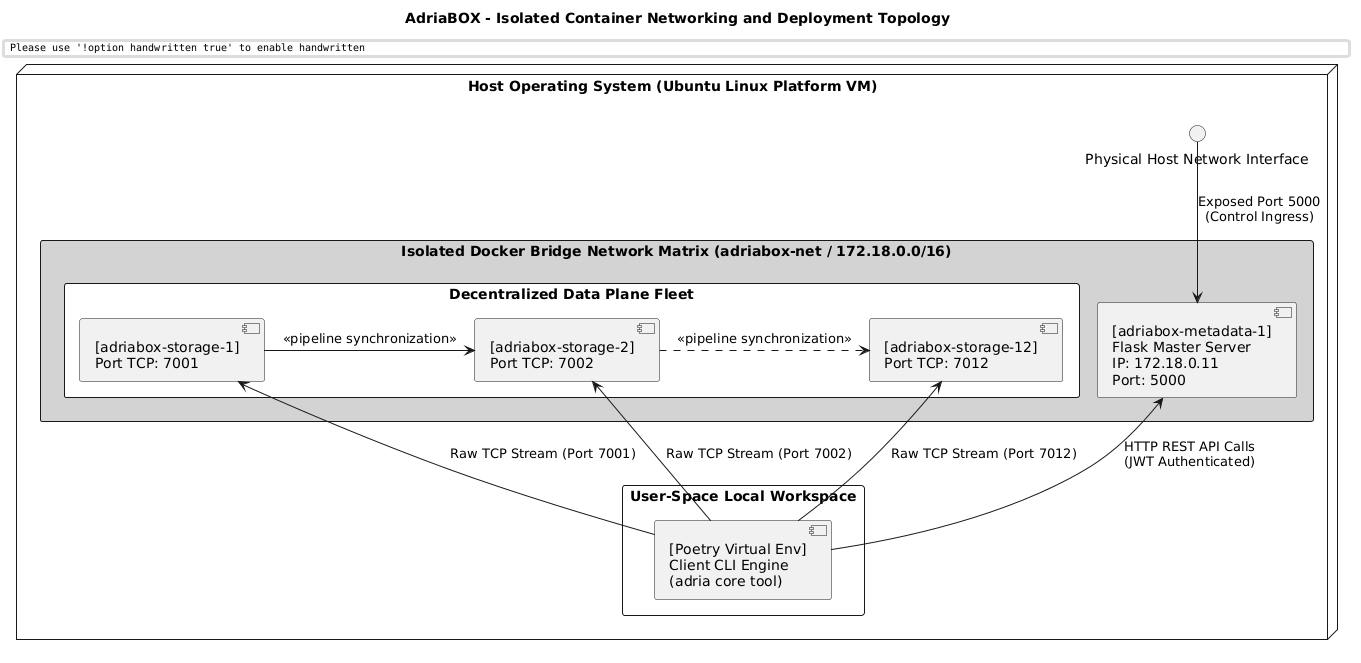
\includegraphics[width=0.95\textwidth]{plantuml/018-container-topology.png}
    \caption{AdriaBOX Deployment Network Topology, Container Partition Boundaries, and Port Mapping Layout.}
    \label{fig:container_topology}
\end{figure}

\subsection{Architectural Paradigm: Simulated vs Production-Grade Cluster}
To evaluate the distributed mechanisms of AdriaBOX on a single physical development machine, the infrastructure is engineered as an orchestrated local multi-container virtualization layer. It is critical to differentiate this validation setup from a real-world enterprise production deployment:

\begin{enumerate}
    \item \textbf{Network Isolation vs WAN Routing:} In this validation environment, network isolation is achieved using a single virtual Docker bridge network (\texttt{adriabox-net} on subnet \texttt{172.18.0.0/16}). In a market-ready infrastructure, each storage node and the metadata master would run on physically distinct bare-metal servers distributed across multiple geographic Availability Zones, communicating over TLS-encrypted Wide Area Network (WAN) channels protected by dedicated firewalls and security groups.
    \item \textbf{Storage Sandboxing vs Distributed Block Storage:} To simulate independent disks, the storage daemons leverage host volume sandboxing (\texttt{./storage\_data/nodeX}), segmenting distinct directories on the same physical hard drive. A real enterprise production environment would utilize actual isolated block devices or dedicated cryptographic NVMe arrays mapped directly to each independent machine node to prevent localized hardware single points of failure (SPOF).
    \item \textbf{Port Demultiplexing vs Standard Service Binding:} Because all nodes coexist on a single host IP during this validation phase, their internal listening port (\texttt{5001}) must be sequentially mapped to distinct host interfaces (\texttt{7001} through \texttt{7012}). On a production market deployment, this artificial demultiplexing is removed: every node binds natively to standard system ports (e.g., HTTPS \texttt{443}), as each server possesses its own distinct public or private IPv4/IPv6 address.
\end{enumerate}

\subsection{Engineering the Multi-Container Deployment Script}
To manage the multi-node storage configuration without manual process execution, the system architecture utilizes a customized, multi-tier orchestration file: \texttt{docker-compose.yml}. Instead of stacking definitions redundantly, the orchestration layer applies YAML extensions and anchor blocks (\texttt{\&storage-base}) to instantiate the 12 independent, decoupled storage container daemons deterministically.

\begin{lstlisting}[basicstyle=\small\ttfamily, frame=single, keepspaces=true, columns=flexible]
version: "3.8"

networks:
  adriabox-net:
    driver: bridge
    ipam:
      config:
        - subnet: 172.18.0.0/16

x-storage-template: &storage-base
  build:
    context: .
    dockerfile: Dockerfile.storage
  networks:
    - adriabox-net
  restart: on-failure

services:
  metadata:
    build:
      context: .
      dockerfile: Dockerfile.metadata
    ports:
      - "5000:5000"
    volumes:
      - metadata-db:/app/data
    networks:
      adriabox-net:
        ipv4_address: 172.18.0.11
    env_file: .env

  storage1:
    <<: *storage-base
    ports:
      - "7001:5001"
    volumes:
      - ./storage_data/node1:/app/storage/storage1
    environment:
      - NODE_ID=storage1

  storage2:
    <<: *storage-base
    ports:
      - "7002:5001"
    volumes:
      - ./storage_data/node2:/app/storage/storage2
    environment:
      - NODE_ID=storage2
\end{lstlisting}

This orchestration structure guarantees the following multi-tenant primitives:
\begin{enumerate}
    \item \textbf{Isolated Control Ingress:} The metadata service has an invariant, static virtual IP (\texttt{172.18.0.11}) inside the bridge network, separating management tasks from the data routing layers.
    \item \textbf{Decoupled Port Allocation:} Each storage node maps its internal listening configuration (\texttt{5001}) to sequential, dedicated host interface targets (\texttt{7001} up to \texttt{7012}) to avoid host interface conflicts.
    \item \textbf{Host Volume Sandboxing:} Persistent directories are segregated on the host machine filesystem (\texttt{./storage\_data/nodeX}). This configuration prevents cross-node block pollution and simulates separate, isolated storage domains on disk.
\end{enumerate}

\subsection{IT-Manager Horizon: Infrastructure Step-by-Step Installation}
This section details the sequential execution manual for the system administrator to initialize the backend distributed infrastructure cluster from an unconfigured state on the core host terminal.

\subsubsection{Step 1: Code Base Extraction}
Clone the clean code repository from the version control platform and navigate into the target workspace:
\begin{lstlisting}[language=bash, keepspaces=true, columns=flexible]
$ git clone https://github.com/wearemassive78/AdriaBOX.git
$ cd AdriaBOX/
\end{lstlisting}

\subsubsection{Step 2: Cryptographic Key Generation and Environment Provisioning}
Before generating the runtime configuration file, a cryptographically secure, high-entropy 256-bit hexadecimal token must be generated. This token acts as the primary secret key for computing and validating HMAC-SHA256 signatures on JSON Web Tokens (JWT), preventing identity spoofing across the network. The system administrator utilizes OpenSSL to derive this key:
\begin{lstlisting}[language=bash, keepspaces=true, columns=flexible]
$ openssl rand -hex 32
9a82f3c1d4e5f6a7b8c9d0e1f2a3b4c5d6e7f8a9b0c1d2e3f4a5b6c7d8e9f0a2
\end{lstlisting}

Using the generated key, the operator creates the definitive \texttt{.env} file at the repository root directory. This configuration acts as the centralized source of truth for the environment:
\begin{minipage}{\linewidth}
\begin{lstlisting}[language=bash, keepspaces=true, columns=flexible]
$ cat <<EOF > .env
ADRIABOX_ENV=production
METADATA_SERVER_HOST=0.0.0.0
METADATA_SERVER_PORT=5000
JWT_SECRET_KEY=9a82f3c1d4e5f6a7b8c9d0e1f2a3b4c5d6e7f8a9b0c1d2e3f4a5b6c7d8e9f0a2
JWT_EXPIRATION_HOURS=24
STORAGE_BIND_ADDRESS=0.0.0.0
STORAGE_INTERNAL_PORT=5001
REPLICATION_FACTOR=3
TOTAL_STORAGE_NODES=12
EOF
\end{lstlisting}
\end{minipage}

The configuration parameters are analyzed below:
\begin{itemize}
    \item \textbf{ADRIABOX\_ENV}: Defines the operational state (\texttt{production}), disabling debugging logs and verbose error displays that could expose system weaknesses.
    \item \textbf{METADATA\_SERVER\_HOST} and \textbf{METADATA\_SERVER\_PORT}: Explicitly bind the central management component to listen across all network interfaces on port \texttt{5000}.
    \item \textbf{JWT\_SECRET\_KEY} and \textbf{JWT\_EXPIRATION\_HOURS}: Establish the core cryptographic boundaries, anchoring the token expiration to 24 hours.
    \item \textbf{STORAGE\_BIND\_ADDRESS} and \textbf{STORAGE\_INTERNAL\_PORT}: Configure the target listener within the internal data plane containers to use port \texttt{5001}.
    \item \textbf{REPLICATION\_FACTOR}: Defines the exact structural duplication factor ($R=3$), meaning each uploaded block will be stored across three separate nodes to ensure fault tolerance.
    \item \textbf{TOTAL\_STORAGE\_NODES}: Sets the total number of sequential worker blocks ($N=12$) tracked within the cluster metadata.
\end{itemize}

\subsubsection{Step 3: Orchestrated Backend Cluster Execution}
Compile the storage and metadata base images, and launch the multi-container topology in background daemon mode:
\begin{lstlisting}[language=bash, keepspaces=true, columns=flexible]
$ sudo docker-compose up --build -d
\end{lstlisting}
The terminal outputs the compilation steps and finishes by creating the isolated networks and worker daemons:
\begin{lstlisting}[basicstyle=\small\ttfamily, breaklines=true, frame=single, keepspaces=true, columns=flexible]
Network adriabox_adriabox-net Created
Container adriabox-storage-1  Started
Container adriabox-storage-12 Started
Container adriabox-metadata-1 Started
\end{lstlisting}

At this point, the server-side architecture control plane is fully deployed and listening for storage client connections.

\subsection{Tenant End-User Horizon: Local Workspace Step-by-Step Installation}
To eliminate local host environment pathfinding issues and guarantee total package isolation on the tenant's workstation, the client workspace is deployed inside a dedicated Docker container running an official \texttt{python:3.12} base image.

Throughout the execution steps of this horizon, the generic lowercase parameters written in italicized form (\textit{username} and \textit{password}) serve as variables that the tenant must substitute with their specific credentials (for example, utilizing usernames such as \texttt{sam}, \texttt{max}, or \texttt{devil}, paired with administrative or user security keys like \texttt{123}, \texttt{321}, or \texttt{666}).

\subsubsection{Step 1: Deploying the Isolated Client Workspace Container}
Run a persistent client container, mapping the project codebase from the host into the internal directory tree, and bind it to the cluster bridge network:
\begin{lstlisting}[language=bash, keepspaces=true, columns=flexible, escapeinside={(*}{*)}]
$ sudo docker run -d --name adriabox-client-(*\textit{username}*) --network adriabox_adriabox-net -e ADRIA_METADATA_URL="http://metadata:5000" -v ~/AdriaBOX:/app -w /app python:3.12 tail -f /dev/null
\end{lstlisting}

This operational layout is structured using the following isolated primitives:
\begin{itemize}
    \item \textbf{--name adriabox-client-}\textit{username}: Defines a dedicated logical label for the workstation environment, separating client executions from the backend services.
    \item \textbf{--network adriabox\_adriabox-net}: Mounts the workspace directly into the cluster virtual bridge backbone, allowing internal name resolution and routing to the metadata service.
    \item \textbf{-e ADRIA\_METADATA\_URL}: Injects the control plane network coordinate directly as an environment variable, pointing to the metadata endpoint container.
    \item \textbf{-v \~{}/AdriaBOX:/app}: Establishes a persistent bidirectional filesystem volume mount. Any change made to the source tree on the host machine is automatically synchronized within the container workspace.
    \item \textbf{tail -f /dev/null}: Serves as a persistent background idle task blocking mechanism. It prevents the container process layout from exiting prematurely, keeping the workspace session constantly active.
\end{itemize}

\subsubsection{Step 2: Entering the Client Container Execution Context}
Access the interactive bash terminal session inside the newly spawned client workspace container:
\begin{lstlisting}[language=bash, keepspaces=true, columns=flexible, escapeinside={(*}{*)}]
$ sudo docker exec -it adriabox-client-(*\textit{username}*) bash
\end{lstlisting}
The host terminal hands over execution control, changing the command prompt context to the root user inside the container:
\begin{lstlisting}[basicstyle=\small\ttfamily, frame=single, keepspaces=true, columns=flexible]
root@e08290fddb49:/app#
\end{lstlisting}

\subsubsection{Step 3: Bootstrapping the Package Manager and Pruning Dependencies}
First, install the modern Poetry orchestration system directly into the clean container operating layer environment:
\begin{lstlisting}[language=bash, keepspaces=true, columns=flexible]
root@e08290fddb49:/app# pip install poetry
\end{lstlisting}
The terminal executes the Python package installer and returns confirmation:
\begin{lstlisting}[basicstyle=\small\ttfamily, breaklines=true, frame=single, keepspaces=true, columns=flexible]
Successfully installed poetry-2.4.1
\end{lstlisting}

Once Poetry is available, invoke the localized project workspace build. Passing the selective \texttt{--without server} flag forces the dependency engine to completely discard web framework libraries like Flask. This keeps the client space slim and fully isolated from backend utilities:
\begin{lstlisting}[language=bash, keepspaces=true, columns=flexible]
root@e08290fddb49:/app# poetry install --without server
\end{lstlisting}
Poetry builds the isolated interpreter path and links the local binaries:
\begin{lstlisting}[basicstyle=\small\ttfamily, breaklines=true, frame=single, keepspaces=true, columns=flexible]
Creating virtualenv adriabox-9TtSrW0h-py3.12 in /root/.cache/pypoetry/virtualenvs
Installing dependencies from lock file
Package operations: 17 installs, 0 updates, 0 removals
Installing the current project: adriabox (0.1.0)
\end{lstlisting}

\subsubsection{Step 4: Client Configuration Anatomy}
The client-side command-line interface discovers network coordinates by loading an external configuration envelope from its local storage partition, located at \texttt{\~{}/.config/adriabox/config.json}. This file is generated automatically by the application upon initializing the first network transaction, but it can be manually written or updated by the tenant to override endpoint destinations:

\begin{lstlisting}[basicstyle=\small\ttfamily, frame=single, keepspaces=true, columns=flexible]
{
  "metadata_endpoint": "http://metadata:5000",
  "default_transfer_chunk_bytes": 4096,
  "socket_timeout_seconds": 15,
  "local_state_storage_path": "~/.config/adriabox/session.json"
}
\end{lstlisting}

The architecture of the JSON fields is defined below:
\begin{itemize}
    \item \textbf{metadata\_endpoint}: The target base network address used by the CLI to route authentication and metadata queries. Within the Docker network, it resolves directly to the metadata service container.
    \item \textbf{default\_transfer\_chunk\_bytes}: Specifies the internal size limit (4 KB) for dividing blocks during cryptographic encryption and network data plane pipelines.
    \item \textbf{socket\_timeout\_seconds}: Enforces a strict network transmission timeout threshold (15 seconds) to prevent communication deadlocks during transfer events.
    \item \textbf{local\_state\_storage\_path}: Defines the specific internal path on the local disk where the runtime engine serializes active user profiles and temporary JWT authorization tokens.
\end{itemize}

\subsection{End-To-End Cluster Integration Handshake Verification}
With both the backend cluster and the tenant workstation running in separate virtual compartments, end-to-end integration and access boundaries are verified.

\subsubsection{Step 1: Tenant Onboarding (Executed Inside the Client Container)}
From the open shell session inside the client container, issue an unauthenticated registration command to onboard the new tenant:
\begin{lstlisting}[language=bash, keepspaces=true, columns=flexible, escapeinside={(*}{*)}]
root@e08290fddb49:/app# poetry run adria register (*\textit{username}*) (*\textit{password}*)
\end{lstlisting}
The client interface communicates with the metadata server through the virtual bridge network, outputting the confirmation trace:
\begin{lstlisting}[basicstyle=\small\ttfamily, frame=single, keepspaces=true, columns=flexible]
+------------------------------------------------------------------------------+
|                              :anchor: AdriaBOX                               |
+------------------------------------------------------------------------------+
A compact CLI for the AdriaBOX project.                                         
Registration successful. Please login.
\end{lstlisting}

\subsubsection{Step 2: Verification and Out-Of-Band Administrative Role Elevation}
To preserve strict system integrity and fulfill fundamental zero-trust cybersecurity primitives, the AdriaBOX control plane intentionally refuses to expose public endpoint routes or API pathways capable of altering user authorization ranks. Allowing role transitions via standard network transactions introduces critical exploitation boundaries, such as broken object-level authorization and privilege escalation vulnerabilities.

Linear role elevation must be prevented; therefore, to elevate a standard tenant to the administrator tier, an infrastructure operator must perform an out-of-band direct database modification. This requires executing a query directly on the isolated metadata storage volume, bypassing the application layer entirely.

First, the user executes the identity tracking command inside the \textbf{client container} to verify their initial status:
\begin{lstlisting}[language=bash, keepspaces=true, columns=flexible]
root@e08290fddb49:/app# poetry run adria login devil 666
root@e08290fddb49:/app# poetry run adria whoami
\end{lstlisting}
The local state engine extracts the unprivileged properties from the active session token, outputting the default role registration matrix:
\begin{lstlisting}[basicstyle=\small\ttfamily, frame=single, keepspaces=true, columns=flexible]
root@e08290fddb49:/app# poetry run adria whoami
+------------------------------------------------------------------------------+
|                              :anchor: AdriaBOX                               |
+------------------------------------------------------------------------------+
A compact CLI for the AdriaBOX project.                                         
devil -- role: user
root@e08290fddb49:/app# 
\end{lstlisting}

To perform the out-of-band role elevation, the operator switches to a separate terminal window on the \textbf{system host machine} and issues an SQL modification command directly to the embedded database engine running inside the active server container:
\begin{lstlisting}[language=bash, keepspaces=true, columns=flexible, escapeinside={(*}{*)}]
$ sudo docker exec -it adriabox-metadata-1 sqlite3 /app/data/metadata.db "UPDATE users SET role = 'admin' WHERE username = '(*\textit{username}*)';"
\end{lstlisting}

\subsubsection{Step 3: Verification of Administrative Cluster Control (Inside Client Container)}
Return to the active terminal window inside the \textbf{client container}. Re-authenticate the newly elevated user session to capture the updated, cryptographically signed JWT payload, and re-execute the identity mapping query to track authorization changes:
\begin{lstlisting}[language=bash, keepspaces=true, columns=flexible]
root@e08290fddb49:/app# poetry run adria login devil 666
root@e08290fddb49:/app# poetry run adria whoami
\end{lstlisting}
The control plane extracts the newly injected administrative privileges, confirming the successful elevation profile:
\begin{lstlisting}[basicstyle=\small\ttfamily, frame=single, keepspaces=true, columns=flexible]
root@e08290fddb49:/app# poetry run adria whoami
+------------------------------------------------------------------------------+
|                              :anchor: AdriaBOX                               |
+------------------------------------------------------------------------------+
A compact CLI for the AdriaBOX project.                                         
devil -- role: admin
root@e08290fddb49:/app# 
\end{lstlisting}

With administrative privileges confirmed, query the restricted status tracking utility to pull down the operational cluster telemetry information:
\begin{lstlisting}[language=bash, keepspaces=true, columns=flexible]
root@e08290fddb49:/app# poetry run adria cluster-status
\end{lstlisting}
The server validates the cryptographic signature of the JWT, recognizes the admin role inside the claims, and opens the restricted instrumentation data path, outputting the live status tracking dashboard matrix:
\begin{lstlisting}[basicstyle=\small\ttfamily, breaklines=true, frame=single, keepspaces=true, columns=flexible]
+------------------------------------------------------------------------------+
|                              :anchor: AdriaBOX                               |
+------------------------------------------------------------------------------+
A compact CLI for the AdriaBOX project.                                         
|  Node       Status  HTTP            TCP             Storage Dir              |
|  storage1   online  storage1:5001   storage1:7001   /app/storage/storage1    |
|  storage2   online  storage2:5001   storage2:7002   /app/storage/storage2    |
|  storage3   online  storage3:5001   storage3:7003   /app/storage/storage3    |
|  storage4   online  storage4:5001   storage4:7004   /app/storage/storage4    |
|  storage5   online  storage5:5001   storage5:7005   /app/storage/storage5    |
|  storage6   online  storage6:5001   storage6:7006   /app/storage/storage6    |
|  storage7   online  storage7:5001   storage7:7007   /app/storage/storage7    |
|  storage8   online  storage8:5001   storage8:7008   /app/storage/storage8    |
|  storage9   online  storage9:5001   storage9:7009   /app/storage/storage9    |
|  storage10  online  storage10:5001  storage10:7010  /app/storage/storage10   |
|  storage11  online  storage11:5001  storage11:7011  /app/storage/storage11   |
|  storage12  online  storage12:5001  storage12:7012  /app/storage/storage12   |
+------------------------------------------------------------------------------+
\end{lstlisting}

This validation matrix confirms complete end-to-end integration: the client successfully traverses isolated virtual interfaces, and the cluster verifies that all 12 decentralized storage node domains are active, healthy, and securely accessible under strict administrative governance.

\subsection{Advanced Deployment Automation and Infrastructure as Code}
To bridge the gap between human-engineered installation procedures and production-grade Infrastructure as Code (IaC) principles, the AdriaBOX orchestration plane integrates deterministic automation scripts. These tools eliminate localized pathfinding defects, automate high-entropy cryptographic key generation, and enforce unified environment provisioning across decentralized runtime horizons. Both scripts are designed to be stored directly within the repository root directory (\texttt{AdriaBOX/}) on the host system.

\subsubsection{Orchestrated Control Plane Provisioning: init\_cluster.sh}
The infrastructure plane instantiation can be condensed into a single non-interactive automation hook. The script \texttt{init\_cluster.sh}, located at the repository root, acts as the primary deployment orchestrator for the IT-Manager, automating cryptographic secret derivation via OpenSSL, environment file compiling, and multi-container daemon initialization:

\begin{lstlisting}[language=bash, basicstyle=\small\ttfamily, frame=single, keepspaces=true, columns=flexible, showspaces=false, showstringspaces=false, breaklines=true]
#!/bin/bash
echo "=== AdriaBOX Infrastructure Automation ==="
echo "Generating secure cryptographic 256-bit JWT secret key..."
JWT_KEY=$(openssl rand -hex 32)

echo "Provisioning .env configuration framework..."
cat <<EOT > .env
ADRIABOX_ENV=production
METADATA_SERVER_HOST=0.0.0.0
METADATA_SERVER_PORT=5000
JWT_SECRET_KEY=${JWT_KEY}
JWT_EXPIRATION_HOURS=24
STORAGE_BIND_ADDRESS=0.0.0.0
STORAGE_INTERNAL_PORT=5001
REPLICATION_FACTOR=3
TOTAL_STORAGE_NODES=12
EOT

echo "Compiling system images and launching decentralized fleet..."
sudo docker-compose up --build -d

echo "=== Cluster Core Infrastructure Online ==="
\end{lstlisting}

This scripted lifecycle execution achieves three foundational validation primitives:
\begin{enumerate}
    \item \textbf{Dynamic Boundary Key Injection:} By leveraging \texttt{openssl rand -hex 32} inline, the system operator guarantees that every independent compilation layout generates a mathematically unique identity tracking secret key, protecting the cluster against hardcoded credential vulnerabilities.
    \item \textbf{Verbatim Configuration Marshalling:} The script utilizes a bounded bash heredoc construct to force explicit variable evaluation and ensure absolute synchronization across the sub-services.
    \item \textbf{Non-Blocking Daemon Compilation:} Passing the decoupled build flags forces Docker Compose to build the binary image layers and detach the logging pipelines immediately, leaving the shell terminal available for monitoring.
\end{enumerate}

\subsubsection{Dynamic Workspace Client Provisioning: setup\_client.sh}
For the Tenant End-User horizon, manual setup routines can introduce container isolation defects and host resource contamination. To mitigate these risks, the interactive script \texttt{setup\_client.sh}, positioned within the repository root, provides automated workspace isolation, virtual environment bootstrapping, and client package compiling based on live input:

\begin{lstlisting}[language=bash, basicstyle=\small\ttfamily, frame=single, keepspaces=true, columns=flexible, showspaces=false, showstringspaces=false, breaklines=true]
#!/bin/bash
echo "=== AdriaBOX Tenant Workspace Provisioning ==="
read -p "Enter the tenant identity name (e.g., sam, devil, max): " USERNAME

if [ -z "$USERNAME" ]; then
    echo "Error: Username cannot be empty."
    exit 1
fi

CONTAINER_NAME="adriabox-client-${USERNAME}"

echo "Deploying isolated target environment container: ${CONTAINER_NAME}..."
sudo docker run -d --name "$CONTAINER_NAME" --network adriabox_adriabox-net -e ADRIA_METADATA_URL="http://metadata:5000" -v ~/AdriaBOX:/app -w /app python:3.12 tail -f /dev/null

echo "Bootstrapping Poetry driver within container context..."
sudo docker exec "$CONTAINER_NAME" pip install poetry

echo "Pruning dependency graph and assembling client-side packages..."
sudo docker exec "$CONTAINER_NAME" poetry install --without server

echo "=== Provisioning Complete. Dropping into interactive shell ==="
sudo docker exec -it "$CONTAINER_NAME" bash
\end{lstlisting}

This multi-tier operational script isolates deployment execution stages into a clear, linear sequence:
\begin{enumerate}
    \item \textbf{Dynamic Parameter Capturing:} The execution reads user parameters dynamically via standard input, enabling the platform operator to spawn unique, isolated client container environments from the same baseline code structure.
    \item \textbf{Containerized Environment Mapping:} The script invokes the Docker engine core to initialize a background interpreter compartment, mapping system host partitions dynamically and binding it to the local cluster virtual core network backbone.
    \item \textbf{Out-of-Band Dependency Resolution:} By leveraging targeted encapsulation primitives, the script drives package loading procedures directly within the virtual user-space partition, completely bypassing the host filesystem.
    \item \textbf{Interactive Terminal Handover:} As a final step, the automation maps standard input streams to drop the user session directly into the active root shell prompt of the container, ready to process runtime platform commands.
\end{enumerate}
